\documentclass[11pt,a4paper]{article}

\usepackage[margin=1in]{geometry}
\usepackage{mathptmx}
\usepackage{amsmath}
\usepackage{amssymb}
\usepackage{amsthm}
\usepackage{braket}
\usepackage{tikz}
\usepackage{quantikz}
\usepackage{enumitem}
\usepackage{hyperref}
\usepackage{xcolor}

\definecolor{circuitblue}{RGB}{40,80,160}

\hypersetup{
    colorlinks=true,
    linkcolor=circuitblue,
    urlcolor=circuitblue,
    citecolor=circuitblue
}

\theoremstyle{definition}
\newtheorem{definition}{Definition}[section]
\newtheorem{example}{Example}[section]
\newtheorem{theorem}{Theorem}[section]

\theoremstyle{remark}
\newtheorem*{intuition}{Intuition}
\newtheorem*{keypoint}{Key Point}

\pagestyle{plain}

\setlength{\parindent}{0pt}
\setlength{\parskip}{6pt}

\begin{document}

\begin{center}
    {\LARGE \textbf{Capacity, Power, and Future of QML}}\\[8pt]
    {\large QML}\\[12pt]
    \hrule
\end{center}

\vspace{12pt}
\tableofcontents
\newpage

%% ========================================================
\section{Overview}
%% ========================================================

this is the last lecture. and its the most important one.

for 19 lectures we've built up the tools of quantum machine learning: variational circuits, quantum kernels, quantum classifiers, quantum generative models, error mitigation, the whole stack. now we need to be honest about wt it all means.

the central question: \textbf{does quantum machine learning actually help?}

the answer is nuanced. there r cases where quantum advantage is provably real, cases where its been disproven (dequantized), cases where we genuinely dont know, and cases where people r being... optimistic. this lecture lays out the evidence honestly.

well cover the theoretical foundations (expressibility, capacity, generalization), the dequantization threat, the proven advantages, the unproven hopes, and wt the future might look like. well also hear from some of the sharpest critics in the field --- particularly maria schuld, who has done more than almost anyone to keep the QML community honest.

then well wrap up the entire course: 20 lectures of quantum machine learning, from qubits to barren plateaus to Born machines. lets go.

%% ========================================================
\section{Expressibility and Capacity of Quantum Models}
%% ========================================================

the first question about any ML model: wt can it represent?

\subsection{Expressibility of PQCs}

\begin{definition}[Expressibility]
the expressibility of a PQC is a measure of how well it can cover the space of possible unitaries (or states). formally, it quantifies the distance between the distribution of states generated by the PQC (with random parameters) and the uniform (Haar) distribution over states.
\end{definition}

sim et al. (2019) introduced the expressibility measure:
\[
\text{Expr} = D_{KL}\left(\hat{P}_{\text{PQC}}(F) \| P_{\text{Haar}}(F)\right)
\]
where $F = |\braket{\psi_1 | \psi_2}|^2$ is the fidelity between two randomly sampled states from the PQC, $\hat{P}_{\text{PQC}}(F)$ is the distribution of fidelities from the PQC, and $P_{\text{Haar}}(F)$ is the distribution under Haar-random unitaries.

low expressibility score = the PQC can reach a wide range of states. high score = its stuck in a small corner of Hilbert space.

\begin{intuition}
think of expressibility as ``how much of the Hilbert space can this circuit explore?'' a circuit with only $R_Y$ gates and no entanglement can only produce product states --- a tiny fraction of all possible states. add entangling gates and more layers, and u can reach more of the space.
\end{intuition}

but heres the catch: high expressibility is \emph{not} always good.

\begin{keypoint}
a maximally expressible circuit (one that can reach all unitaries) is also maximally susceptible to barren plateaus. the same property that lets it represent any function also means most of the parameter landscape is flat. theres a fundamental tension between expressibility and trainability.
\end{keypoint}

\subsection{Effective Dimension}

abbas et al. (2021) introduced a more sophisticated measure: the effective dimension.

\begin{definition}[Effective Dimension]
the effective dimension of a quantum model $f(\boldsymbol{\theta}, \mathbf{x})$ with $d$ parameters is:
\[
d_{\text{eff}}(n) = \frac{2 \log\left(\frac{1}{d} \sum_{i=1}^{d} \sqrt{1 + \frac{n}{2\pi \ln n} \lambda_i}\right)}{\log\left(\frac{n}{2\pi \ln n}\right)}
\]
where $\lambda_1, \ldots, \lambda_d$ r the eigenvalues of the normalized Fisher information matrix $\hat{F}$, and $n$ is the number of data samples.
\end{definition}

the Fisher information matrix captures how sensitively the model output depends on each parameter:
\[
F_{ij}(\boldsymbol{\theta}) = \mathbb{E}_{\mathbf{x}}\left[\frac{\partial \log p(y|\mathbf{x}, \boldsymbol{\theta})}{\partial \theta_i} \frac{\partial \log p(y|\mathbf{x}, \boldsymbol{\theta})}{\partial \theta_j}\right]
\]

\begin{intuition}
the effective dimension tells u how many of ur parameters r actually doing useful work. if u have 100 parameters but the effective dimension is 10, then 90 of ur parameters r redundant --- they r just moving the model around in a low-dimensional submanifold.
\end{intuition}

\subsection{Abbas et al. 2021 --- Key Results}

the paper ``the power of quantum neural networks'' made several important findings:

\begin{enumerate}[label=\arabic*.]
    \item quantum models can achieve higher effective dimension than classical models with the same number of parameters. this suggests they make better use of their parameters.

    \item the effective dimension grows with circuit depth and entanglement, up to a point. beyond that point, adding more structure doesnt help (and can hurt trainability).

    \item on specific problems (constructed to favor quantum), the quantum model outperformed classical models with matched effective dimension.

    \item the Fisher information matrix of quantum models has a more uniform spectrum than classical models, suggesting better parameter utilization.
\end{enumerate}

\begin{keypoint}
the takeaway from abbas et al.: quantum models r not just ``bigger'' than classical models --- they use their parameters more efficiently. but this efficiency advantage is problem-dependent, and its not clear that it translates to practical advantage on real-world tasks.
\end{keypoint}

%% ========================================================
\section{VC Dimension of Quantum Classifiers}
%% ========================================================

the VC dimension is the classical measure of model capacity.

\begin{definition}[VC Dimension]
the VC dimension of a binary classifier is the largest set of points that it can shatter (i.e., correctly classify for all possible labelings). formally, $\text{VC}(f) = \max\{m : \exists S \text{ with } |S| = m \text{ that } f \text{ shatters}\}$.
\end{definition}

\begin{theorem}[VC Dimension of Quantum Classifiers]
for a quantum classifier with $d$ trainable parameters acting on $n$ qubits:
\begin{enumerate}[nosep]
    \item upper bound: $\text{VC} \leq O(d \cdot n)$ (bu et al. 2022)
    \item lower bound: $\text{VC} \geq \Omega(d)$ for generic circuits
    \item for circuits with $L$ layers of single-qubit gates and CNOT entanglers: $\text{VC} = \Theta(d)$ where $d = O(n \cdot L)$
\end{enumerate}
\end{theorem}

comparison with classical:
\begin{itemize}[nosep]
    \item linear classifier on $\mathbb{R}^d$: $\text{VC} = d + 1$
    \item neural network with $W$ weights: $\text{VC} = O(W \log W)$
    \item quantum classifier with $d$ parameters: $\text{VC} = O(d \cdot n)$
\end{itemize}

the factor of $n$ in the quantum upper bound is interesting --- it means each quantum parameter can effectively contribute more to the model's capacity than a classical parameter. this is bcs quantum parameters control rotations in exponentially large Hilbert spaces.

\begin{example}
a quantum classifier with $d = 20$ parameters on $n = 5$ qubits has VC dimension up to $O(100)$. a classical linear model needs 100 parameters to match this. thats a 5x compression ratio. but a classical neural network with clever architecture might also achieve compression, so this isnt automatically an advantage.
\end{example}

%% ========================================================
\section{Generalization Bounds}
%% ========================================================

knowing wt a model can represent is one thing. knowing whether it generalizes (performs well on unseen data) is another.

\subsection{Caro et al. 2022}

the paper ``generalization in quantum machine learning from few training data'' gives the tightest known bounds.

\begin{theorem}[Quantum Generalization Bound (Caro et al. 2022)]
for a quantum classifier with $T$ trainable gates, trained on $N$ data points, the expected prediction error on new data satisfies:
\[
\text{error}_{\text{test}} \leq \text{error}_{\text{train}} + O\left(\sqrt{\frac{T \log T}{N}}\right)
\]
with high probability over the random training set.
\end{theorem}

this looks very similar to classical generalization bounds (like Rademacher complexity bounds), and thats the point: quantum models generalize in essentially the same way as classical models.

\begin{keypoint}
the generalization bound depends on $T$ (number of trainable gates), not on the Hilbert space dimension $2^n$. this is crucial: even though the model ``lives'' in an exponentially large space, its complexity (for generalization purposes) is controlled by the number of parameters, not the space dimension.
\end{keypoint}

implications:
\begin{enumerate}[label=\arabic*.]
    \item u dont need exponentially many training samples to train a quantum model. $N = O(T \log T)$ samples suffice.
    \item adding more qubits (increasing $n$) doesnt automatically hurt generalization, as long as the number of gates stays controlled.
    \item the bound is agnostic to whether the data is classical or quantum.
\end{enumerate}

\subsection{Beyond Worst-Case Bounds}

the caro et al. bound is worst-case. in practice, quantum models often generalize better than the bound suggests, especially when:
\begin{itemize}[nosep]
    \item the data has quantum structure (e.g., it comes from a quantum process)
    \item the circuit architecture is matched to the problem symmetry
    \item the effective dimension is much smaller than the parameter count
\end{itemize}

\begin{example}
for a classification task on 4 qubits with a 2-layer circuit ($T = 24$ gates), the generalization bound gives: need $N \gtrsim 24 \log 24 \approx 76$ training samples. in practice, the model might generalize well with even fewer samples if the task is structured.
\end{example}

%% ========================================================
\section{The Dequantization Threat}
%% ========================================================

now for the scary part. dequantization is wt happens when a claimed quantum speedup turns out to be achievable classically.

\subsection{Tang 2019 --- Quantum Recommendation Dequantized}

the most famous dequantization result. the background:

\begin{enumerate}[label=\arabic*.]
    \item kerenidis and prakash (2016) showed that quantum computers could do recommendation (like Netflix-style collaborative filtering) exponentially faster than the best known classical algorithm
    \item this was a major result --- one of the few exponential quantum speedups for a practical ML problem
    \item then ewin tang (2019), as an \emph{undergraduate}, showed that a classical algorithm with ``quantum-inspired'' sampling could match the quantum speedup (up to polynomial factors)
\end{enumerate}

\begin{theorem}[Tang's Dequantization]
given sampling and query access to a matrix $A$ (the user-item matrix), there exists a classical algorithm for recommendation that runs in time $\text{poly}(k, 1/\epsilon, \|A\|_F / \sigma_k)$ --- independent of the matrix dimensions. this matches the quantum algorithm's scaling.
\end{theorem}

the key idea: if u have the ability to sample from rows/columns of the matrix proportional to their norms (which is wt quantum amplitude encoding gives u), then u can simulate this classically using ``sample and query'' data structures.

\begin{keypoint}
tangs result didnt just kill one quantum speedup --- it established a general technique. the same approach has since been used to dequantize quantum PCA, quantum supervised learning, and several other quantum ML algorithms. the pattern: any quantum algorithm that relies on amplitude encoding (loading classical data into quantum amplitudes) is vulnerable to dequantization.
\end{keypoint}

\subsection{The Pattern of Dequantization}

since tang 2019, the following quantum ML algorithms have been partially or fully dequantized:
\begin{itemize}[nosep]
    \item quantum recommendation systems (tang 2019)
    \item quantum PCA (tang 2021)
    \item quantum supervised learning / least-squares (gilyen et al. 2022)
    \item quantum Boltzmann machine sampling (certain cases)
\end{itemize}

the common thread: these algorithms all assume that classical data is loaded into quantum states via amplitude encoding. the dequantization shows that if u can do amplitude encoding (which takes $O(2^n)$ time classically), u can also do the computation classically in comparable time.

\begin{intuition}
its like claiming u can sort a list faster with a quantum computer, but only if someone first gives u the list in a special quantum format. if creating that format takes as long as just sorting the list classically, the speedup is illusory.
\end{intuition}

this doesnt mean all quantum ML is doomed. it means we need to be very careful about where the speedup actually comes from.

%% ========================================================
\section{Where Quantum Advantage IS Proven}
%% ========================================================

despite dequantization, there r genuine quantum advantages. lets be precise about wt they r.

\subsection{Liu et al. 2021 --- Rigorous Advantage on Constructed Problems}

\begin{theorem}[Liu, Arunachalam, Temme 2021]
there exists a classification problem based on the discrete logarithm that:
\begin{enumerate}[nosep]
    \item can be solved efficiently by a quantum kernel method (polynomial time)
    \item cannot be solved by any classical learner in polynomial time (under standard cryptographic assumptions)
\end{enumerate}
\end{theorem}

the construction:
\begin{itemize}[nosep]
    \item the data is labeled by a function related to the discrete logarithm
    \item a quantum feature map based on Shor's algorithm can separate the classes
    \item no efficient classical algorithm can compute this feature (unless discrete log is easy, which would break RSA)
\end{itemize}

\begin{keypoint}
this is a real, provable quantum advantage for a machine learning task. but the problem is \emph{constructed} specifically to be hard for classical computers. its not a natural ML problem that arose from practice. the question remains: r there natural problems where quantum helps?
\end{keypoint}

\subsection{Huang et al. 2022 --- Learning Quantum Systems}

\begin{theorem}[Quantum Advantage for Learning Quantum States]
for the task of predicting properties of quantum states:
\begin{itemize}[nosep]
    \item with classical data processing: need $\exp(n)$ measurements of the quantum state
    \item with quantum data processing (quantum memory): need $O(\text{poly}(n))$ measurements
\end{itemize}
this is an exponential quantum advantage.
\end{theorem}

the key insight: if ur data is quantum (actual quantum states), then quantum processing has a provable exponential advantage. this makes physical sense --- trying to characterize a quantum state classically requires exponential resources (quantum state tomography), but a quantum computer can process the state directly.

applications:
\begin{itemize}[nosep]
    \item characterizing quantum devices (quantum process tomography)
    \item predicting molecular properties from quantum simulations
    \item quantum error correction (learning noise models)
    \item quantum sensor data processing
\end{itemize}

\begin{intuition}
the clearest quantum advantage is for quantum data. classical data on quantum hardware is where things get murky. quantum data on quantum hardware is where the advantage is real and provable.
\end{intuition}

\subsection{Other Proven Advantages}

\begin{enumerate}[label=\arabic*.]
    \item \textbf{quantum simulation}: learning properties of quantum many-body systems is exponentially faster with quantum computers (follows from BQP $\neq$ BPP, widely believed).

    \item \textbf{shadow tomography}: predicting many properties of an unknown quantum state using few measurements (aaronson 2018, huang et al. 2020).

    \item \textbf{quantum PAC learning}: for concept classes defined by quantum circuits, quantum learners can be exponentially more efficient (arunachalam and de wolf, 2017).
\end{enumerate}

%% ========================================================
\section{Where Quantum Advantage is NOT Proven}
%% ========================================================

now the uncomfortable part. for most of wt people actually mean by ``QML,'' quantum advantage is not proven.

\subsection{Classical Data, NISQ Hardware}

the majority of QML research uses:
\begin{itemize}[nosep]
    \item classical datasets (MNIST, iris, etc.)
    \item variational quantum circuits on NISQ hardware
    \item hybrid quantum-classical optimization
\end{itemize}

for this setting, there is \textbf{no proven quantum advantage}. the reasons:

\begin{enumerate}[label=\arabic*.]
    \item \textbf{data encoding bottleneck}: encoding $N$ classical data points into quantum states takes at least $O(N)$ time. any computation on the quantum side has to beat this overhead.

    \item \textbf{limited circuit depth}: NISQ hardware limits circuit depth to $\sim 100$ gates. this severely constrains wt quantum operations u can do.

    \item \textbf{classical ML is really good}: modern classical methods (deep learning, gradient boosting, kernel methods) r extremely powerful. beating them on classical data with noisy quantum circuits is a tall order.

    \item \textbf{barren plateaus}: as we discussed in lecture 14, variational circuits suffer from exponentially vanishing gradients, which limits scalability.
\end{enumerate}

\subsection{Numerical Evidence}

many papers show quantum models performing comparably to (or slightly worse than) classical models on standard benchmarks:
\begin{itemize}[nosep]
    \item MNIST: classical CNNs achieve $>99\%$ accuracy. best quantum results: $\sim 95$--$98\%$ with significant overhead.
    \item iris dataset: both classical and quantum achieve $\sim 97\%$ accuracy, but the quantum version is much slower.
    \item molecular property prediction: classical GNNs r competitive with or better than quantum approaches for the datasets tested so far.
\end{itemize}

\begin{keypoint}
the absence of proven advantage doesnt mean advantage is impossible. it means we havent found it yet for classical data tasks. the search continues, and there r good theoretical reasons to think advantage might exist for certain structured problems.
\end{keypoint}

%% ========================================================
\section{Fault-Tolerant QML}
%% ========================================================

everything changes with error correction.

\subsection{What Error Correction Gives Us}

fault-tolerant quantum computers can run circuits of arbitrary depth without accumulating errors. this unlocks:

\begin{enumerate}[label=\arabic*.]
    \item \textbf{HHL algorithm}: solve systems of linear equations $A\mathbf{x} = \mathbf{b}$ in time $O(\text{poly}(\log N, \kappa))$ where $N$ is the dimension and $\kappa$ is the condition number. this is exponentially faster than classical for certain matrices.

    \item \textbf{quantum linear algebra}: matrix inversion, eigenvalue estimation, singular value transformation --- all with exponential speedups in certain regimes.

    \item \textbf{deep quantum circuits}: can implement quantum algorithms (Grover's, quantum walks, etc.) that require coherent execution of many gates.

    \item \textbf{quantum RAM (qRAM)}: with fault tolerance, qRAM becomes feasible (in principle), unlocking the speedups that currently require amplitude encoding.
\end{enumerate}

\begin{definition}[Quantum RAM]
quantum RAM (qRAM) is a quantum device that can query a classical database in superposition:
\[
\text{qRAM}: \sum_i \alpha_i \ket{i}\ket{0} \to \sum_i \alpha_i \ket{i}\ket{x_i}
\]
where $x_i$ is the $i$-th database entry. this enables coherent quantum access to classical data.
\end{definition}

\subsection{The qRAM Problem}

\begin{keypoint}
many quantum speedups for classical data require qRAM. but qRAM is extremely challenging to build. it needs $O(N)$ quantum switches for a database of size $N$, each of which must maintain coherence. no one has built a practical qRAM yet, and its unclear when (or if) we will.
\end{keypoint}

without qRAM, the cost of loading classical data into quantum states is $O(N)$, which often negates the quantum speedup. this is the fundamental bottleneck for quantum ML on classical data.

the situation in table form:

\begin{center}
\renewcommand{\arraystretch}{1.4}
\begin{tabular}{|p{4cm}|p{4cm}|p{4cm}|}
\hline
\textbf{Setting} & \textbf{With qRAM} & \textbf{Without qRAM} \\
\hline
linear systems (HHL) & exponential speedup & no speedup (loading bottleneck) \\
\hline
quantum PCA & exponential speedup & dequantized (tang) \\
\hline
quantum recommendation & exponential speedup & dequantized (tang) \\
\hline
quantum SVM & polynomial speedup & no clear advantage \\
\hline
quantum kernel methods & potential advantage & problem-dependent \\
\hline
\end{tabular}
\end{center}

\subsection{Fault-Tolerant Timeline}

when will we have fault-tolerant quantum computers? current estimates:
\begin{itemize}[nosep]
    \item logical qubits available: $\sim$2026--2028 (first demonstrations)
    \item $\sim 100$ logical qubits: $\sim$2028--2032
    \item enough for practical HHL: $\sim$thousands of logical qubits, likely 2032+
    \item practical qRAM: unclear, possibly much later
\end{itemize}

so fault-tolerant QML is a medium to long-term prospect. NISQ QML is wt we have now.

%% ========================================================
\section{Quantum Data vs Classical Data}
%% ========================================================

this distinction is crucial and often glossed over.

\begin{definition}[Quantum Data]
data that is naturally quantum --- i.e., it consists of quantum states that come from a quantum process (a quantum computer, a quantum sensor, a quantum communication channel). the data cannot be efficiently represented classically.
\end{definition}

\begin{definition}[Classical Data]
data that can be written down as classical bits (numbers, images, text, etc.). most real-world ML data is classical.
\end{definition}

the advantage landscape:

\begin{center}
\renewcommand{\arraystretch}{1.4}
\begin{tabular}{|p{4cm}|p{4.5cm}|p{4.5cm}|}
\hline
 & \textbf{Quantum processor} & \textbf{Classical processor} \\
\hline
\textbf{Quantum data} & natural fit, proven exponential advantages (Huang et al. 2022) & exponentially wasteful (need tomography) \\
\hline
\textbf{Classical data} & unclear advantage, loading bottleneck, dequantization threat & well-developed, highly optimized \\
\hline
\end{tabular}
\end{center}

\begin{keypoint}
the clearest path to quantum advantage in ML is through quantum data. as quantum computers, quantum sensors, and quantum networks become more common, there will be more quantum data to process. classical data on quantum hardware remains the hardest case to justify.
\end{keypoint}

%% ========================================================
\section{Maria Schuld's Critical Perspective}
%% ========================================================

maria schuld (xanadu, university of KwaZulu-Natal) has been one of the most thoughtful and honest voices in QML. her perspective deserves a dedicated section.

\subsection{Quantum Models Are Kernel Methods}

schuld's key insight (schuld 2021, ``supervised quantum machine learning models are kernel methods''):

\begin{theorem}[Schuld 2021]
any quantum model of the form $f(\mathbf{x}) = \bra{0} U^\dagger(\mathbf{x}) M U(\mathbf{x}) \ket{0}$, where $U(\mathbf{x})$ is a data-encoding unitary and $M$ is a measurement operator, can be written as:
\[
f(\mathbf{x}) = \sum_i \alpha_i k(\mathbf{x}_i, \mathbf{x}) + b
\]
for some kernel function $k(\mathbf{x}, \mathbf{x}') = |\bra{0} U^\dagger(\mathbf{x}) U(\mathbf{x}') \ket{0}|^2$.
\end{theorem}

this means that variational quantum classifiers r mathematically equivalent to kernel methods. the quantum circuit defines a feature map into Hilbert space, and the classification is linear in that feature space.

\begin{intuition}
this is both liberating and sobering. liberating bcs it connects QML to a well-understood classical framework. sobering bcs kernel methods r well-studied, and we know their limitations. if quantum models r ``just'' kernel methods, then the advantage has to come from the specific kernel being quantum-hard to compute classically.
\end{intuition}

\subsection{The Importance of Honesty}

schuld has argued (and i agree) that the QML community needs to be more honest about:

\begin{enumerate}[label=\arabic*.]
    \item \textbf{benchmarking}: comparing quantum models to properly tuned classical baselines, not strawman classicals.

    \item \textbf{scaling}: showing that quantum models scale to meaningful problem sizes, not just toy examples on 4 qubits.

    \item \textbf{advantage claims}: being precise about wt ``advantage'' means --- is it computational (speedup), statistical (better generalization), or practical (easier to implement)?

    \item \textbf{the loading problem}: acknowledging that encoding classical data into quantum states is expensive and often negates any quantum advantage.

    \item \textbf{purpose}: asking ``why quantum?'' for each application, not just ``can we make it quantum?''
\end{enumerate}

\begin{keypoint}
schuld's perspective: QML is a legitimate scientific endeavor, but it needs intellectual honesty. claiming advantage without evidence hurts the field. the most productive direction is understanding \emph{when} and \emph{why} quantum helps, not trying to make everything quantum.
\end{keypoint}

%% ========================================================
\section{Future Directions}
%% ========================================================

where is QML going? heres my honest assessment.

\subsection{Quantum Transfer Learning}

\begin{definition}[Quantum Transfer Learning]
use a pre-trained classical model (e.g., a CNN) for feature extraction, then use a small quantum circuit for the final classification/regression on those features. the classical part handles the heavy lifting; the quantum part adds expressivity in the final feature space.
\end{definition}

this is pragmatic: u dont try to replace the whole classical pipeline, just augment the last layer. mari et al. (2020) showed this can work for image classification.

the circuit:
\begin{center}
\begin{quantikz}
\lstick{$\ket{0}$} & \gate{R_Y(x_1)} & \ctrl{1} & \gate{R_Y(\theta_1)} & \ctrl{1} & \meter{} \\
\lstick{$\ket{0}$} & \gate{R_Y(x_2)} & \targ{} & \gate{R_Y(\theta_2)} & \targ{} & \meter{} \\
\lstick{$\ket{0}$} & \gate{R_Y(x_3)} & \ctrl{1} & \gate{R_Y(\theta_3)} & \ctrl{1} & \meter{} \\
\lstick{$\ket{0}$} & \gate{R_Y(x_4)} & \targ{} & \gate{R_Y(\theta_4)} & \targ{} & \meter{}
\end{quantikz}
\end{center}

where $x_1, \ldots, x_4$ r features extracted by a classical CNN. the quantum circuit then classifies based on these features.

\subsection{Quantum Natural Language Processing}

this is one of the wilder directions. the idea (coecke, sadrzadeh, clark 2010; meichanetzidis et al. 2020):

\begin{enumerate}[label=\arabic*.]
    \item natural language has compositional structure (words combine to form sentences according to grammatical rules)
    \item this structure can be formalized using category theory (specifically, pregroup grammars)
    \item quantum mechanics also has compositional structure (tensor products, composition of maps)
    \item the mathematical frameworks r the same! (both r compact closed categories)
    \item so: map linguistic structure to quantum circuits, where words r quantum states and grammatical composition is tensor product
\end{enumerate}

this is the DisCoCat (Distributional Compositional Categorical) framework.

\begin{example}
the sentence ``Alice likes Bob'' maps to:
\begin{itemize}[nosep]
    \item ``Alice'' $\to$ state $\ket{\psi_A}$ on one qubit
    \item ``likes'' $\to$ a two-qubit operation (maps subject and object to a meaning)
    \item ``Bob'' $\to$ state $\ket{\psi_B}$ on one qubit
\end{itemize}
the sentence meaning is: apply the ``likes'' operation to the tensor product of Alice and Bob states, then measure to get a classification (e.g., sentiment).
\end{example}

its beautiful mathematically. whether it has practical value is still open. the company Quantinuum has done the most work here with their lambeq library.

\subsection{Quantum Reinforcement Learning}

quantum RL combines quantum computing with reinforcement learning:
\begin{itemize}[nosep]
    \item \textbf{quantum environments}: the agent interacts with a quantum system (e.g., controlling a quantum experiment). here quantum advantage is natural bcs the environment is quantum.
    \item \textbf{quantum policies}: use a PQC as the policy network. the Born rule gives stochastic policies naturally.
    \item \textbf{quantum speedup for exploration}: Grover-like quadratic speedup for finding optimal actions in certain settings.
\end{itemize}

jerbi et al. (2021) showed that quantum agents can achieve provable advantages in certain oracle-based RL settings. for practical RL problems, the picture is less clear.

\subsection{Quantum Federated Learning}

distributed ML where quantum devices collaborate without sharing raw quantum data. relevant for:
\begin{itemize}[nosep]
    \item quantum sensor networks
    \item privacy-preserving quantum computation
    \item multi-party quantum machine learning
\end{itemize}

the quantum advantage here comes from quantum communication (e.g., using entanglement to reduce communication costs).

%% ========================================================
\section{The Author's Take}
%% ========================================================

ok time for me to be honest about wt i think.

QML is a fascinating field at the intersection of two of the most exciting areas of science and technology. the mathematical connections between quantum mechanics and machine learning r deep and beautiful. some of the theoretical results (quantum kernel advantages, learning quantum states, expressibility theory) r genuinely important contributions to our understanding.

but --- and this is a big but --- i dont think QML is going to replace classical ML anytime soon. heres why:

\begin{enumerate}[label=\arabic*.]
    \item \textbf{infrastructure first}: before QML can be practical, we need better quantum hardware (more qubits, lower error rates), better compilers (more efficient circuit optimization), and better error correction (to enable fault-tolerant computation). these r hardware and systems challenges, not ML challenges.

    \item \textbf{the classical baseline is a moving target}: classical ML keeps getting better. by the time we have 1000-qubit fault-tolerant machines, classical methods will have advanced too. quantum advantage is relative, not absolute.

    \item \textbf{the loading problem is real}: for classical data, encoding into quantum states is expensive. until we have practical qRAM (which may never happen), this bottleneck limits the applications.

    \item \textbf{quantum data is the sweet spot}: the clearest advantages r for processing quantum data --- characterizing quantum devices, analyzing quantum sensor outputs, learning quantum dynamics. as quantum technology matures, there will be more quantum data, and QML will be essential for processing it.

    \item \textbf{exploration is valuable}: even if practical quantum advantage doesnt materialize in the short term, the research is valuable. it deepens our understanding of both quantum mechanics and machine learning, leads to new classical algorithms (quantum-inspired methods), and trains a workforce for the quantum future.
\end{enumerate}

\begin{keypoint}
my advice: learn QML bcs its intellectually beautiful and bcs quantum computing is coming (eventually). but dont bet ur career on QML solving practical problems in the next 5 years. hedge by being excellent at classical ML too. the people who will make the biggest impact in QML r those who deeply understand both the quantum and the classical sides.
\end{keypoint}

%% ========================================================
\section{Panel Discussion Highlights (QGSS 2021)}
%% ========================================================

the IBM Quantum Global Summer School 2021 had a panel of experts discussing the future of QML. key takeaways:

\begin{enumerate}[label=\arabic*.]
    \item \textbf{kristan temme} (IBM): ``the most important thing is to find the right problems. dont try to quantize everything --- find problems where quantum mechanics gives a natural advantage.''

    \item \textbf{maria schuld}: ``we need to stop comparing 4-qubit quantum circuits to random forests on iris. either we do fair comparisons, or we focus on problems where classical methods genuinely fail.''

    \item \textbf{jarrod mcclean} (Google): ``variational methods r a tool, not a solution. we need to understand when they work and when they dont. barren plateaus r a real obstacle, not just a theoretical curiosity.''

    \item \textbf{amira abbas} (IBM): ``the Fisher information framework gives us a principled way to compare quantum and classical models. lets use it instead of just comparing test accuracies on toy datasets.''

    \item \textbf{consensus view}: QML is worth pursuing, but needs more rigor, better benchmarks, and honest assessment of when quantum helps. the near-term focus should be on understanding, not on overpromising.
\end{enumerate}

%% ========================================================
\section{QML Landscape Map}
%% ========================================================

heres a visual map of the QML field and how its components relate:

\begin{center}
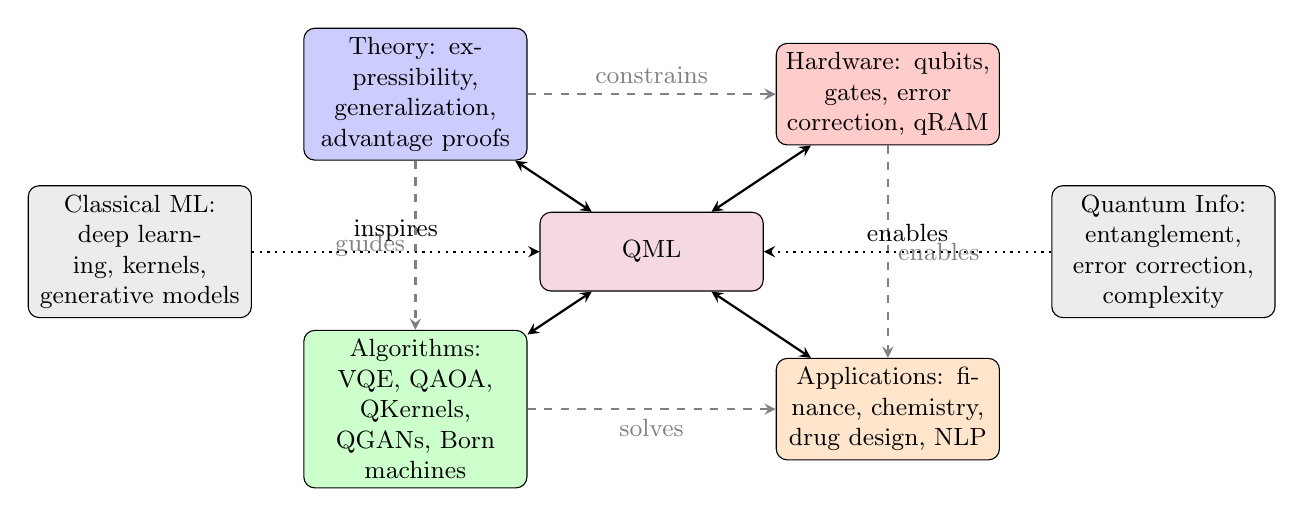
\begin{tikzpicture}[
    box/.style={draw, rounded corners, minimum width=2.8cm, minimum height=1cm, align=center, font=\small, text width=2.6cm},
    arrow/.style={->, thick, >=stealth},
    biarrow/.style={<->, thick, >=stealth},
    every node/.style={font=\small}
]

% Four main pillars
\node[box, fill=blue!20] (theory) at (0, 4) {Theory: expressibility, generalization, advantage proofs};
\node[box, fill=red!20] (hw) at (6, 4) {Hardware: qubits, gates, error correction, qRAM};
\node[box, fill=green!20] (algo) at (0, 0) {Algorithms: VQE, QAOA, QKernels, QGANs, Born machines};
\node[box, fill=orange!20] (app) at (6, 0) {Applications: finance, chemistry, drug design, NLP};

% Center node
\node[box, fill=purple!15, minimum width=2.4cm] (qml) at (3, 2) {QML};

% Connections
\draw[biarrow] (theory) -- (qml);
\draw[biarrow] (hw) -- (qml);
\draw[biarrow] (algo) -- (qml);
\draw[biarrow] (app) -- (qml);

% Cross connections
\draw[arrow, dashed, gray] (theory) -- (algo) node[midway, left] {guides};
\draw[arrow, dashed, gray] (hw) -- (app) node[midway, right] {enables};
\draw[arrow, dashed, gray] (theory) -- (hw) node[midway, above] {constrains};
\draw[arrow, dashed, gray] (algo) -- (app) node[midway, below] {solves};

% External influences
\node[box, fill=gray!15, minimum width=2.4cm] (classml) at (-3.5, 2) {Classical ML: deep learning, kernels, generative models};
\node[box, fill=gray!15, minimum width=2.4cm] (qinfo) at (9.5, 2) {Quantum Info: entanglement, error correction, complexity};

\draw[arrow, dotted] (classml) -- (qml) node[midway, above] {inspires};
\draw[arrow, dotted] (qinfo) -- (qml) node[midway, above] {enables};

\end{tikzpicture}
\end{center}

the four pillars (theory, hardware, algorithms, applications) all feed into each other. classical ML and quantum information theory r the two ``parent fields'' that QML draws from.

%% ========================================================
\section{Timeline of Key QML Results}
%% ========================================================

\begin{center}
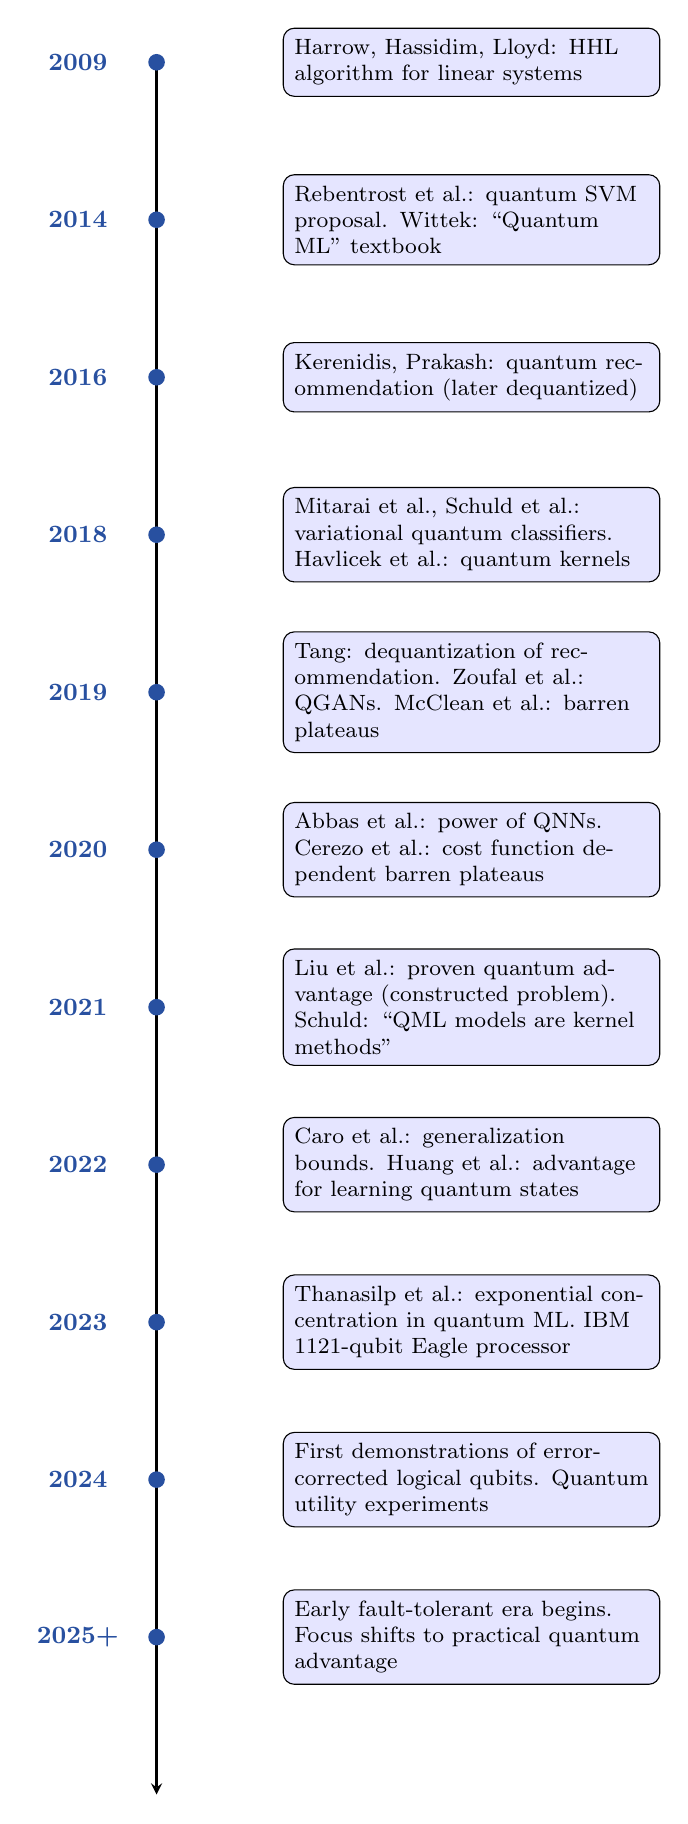
\begin{tikzpicture}[
    every node/.style={font=\footnotesize},
    event/.style={draw, rounded corners, fill=blue!10, text width=4.5cm, align=left, inner sep=4pt},
    year/.style={font=\small\bfseries, text=circuitblue}
]

% Timeline line
\draw[thick, ->, >=stealth] (0, 0) -- (0, -22);

% Events
\node[year] at (-1, 0) {2009};
\node[event] at (4, 0) {Harrow, Hassidim, Lloyd: HHL algorithm for linear systems};

\node[year] at (-1, -2) {2014};
\node[event] at (4, -2) {Rebentrost et al.: quantum SVM proposal. Wittek: ``Quantum ML'' textbook};

\node[year] at (-1, -4) {2016};
\node[event] at (4, -4) {Kerenidis, Prakash: quantum recommendation (later dequantized)};

\node[year] at (-1, -6) {2018};
\node[event] at (4, -6) {Mitarai et al., Schuld et al.: variational quantum classifiers. Havlicek et al.: quantum kernels};

\node[year] at (-1, -8) {2019};
\node[event] at (4, -8) {Tang: dequantization of recommendation. Zoufal et al.: QGANs. McClean et al.: barren plateaus};

\node[year] at (-1, -10) {2020};
\node[event] at (4, -10) {Abbas et al.: power of QNNs. Cerezo et al.: cost function dependent barren plateaus};

\node[year] at (-1, -12) {2021};
\node[event] at (4, -12) {Liu et al.: proven quantum advantage (constructed problem). Schuld: ``QML models are kernel methods''};

\node[year] at (-1, -14) {2022};
\node[event] at (4, -14) {Caro et al.: generalization bounds. Huang et al.: advantage for learning quantum states};

\node[year] at (-1, -16) {2023};
\node[event] at (4, -16) {Thanasilp et al.: exponential concentration in quantum ML. IBM 1121-qubit Eagle processor};

\node[year] at (-1, -18) {2024};
\node[event] at (4, -18) {First demonstrations of error-corrected logical qubits. Quantum utility experiments};

\node[year] at (-1, -20) {2025+};
\node[event] at (4, -20) {Early fault-tolerant era begins. Focus shifts to practical quantum advantage};

% Markers
\foreach \y in {0,-2,-4,-6,-8,-10,-12,-14,-16,-18,-20}
    \fill[circuitblue] (0,\y) circle (3pt);

\end{tikzpicture}
\end{center}

%% ========================================================
\section{Course Summary: 20 Lectures of QML}
%% ========================================================

lets look back at the journey.

\subsection{Part I: Foundations (Lectures 1--5)}

\begin{enumerate}[label=\textbf{Lec \arabic*:}]
    \item \textbf{intro to quantum computing}: qubits, gates, measurements, the computational model. we built the language we'd use for everything else.

    \item \textbf{quantum circuits and universality}: how to build arbitrary unitaries from simple gates. the circuit model of quantum computing.

    \item \textbf{entanglement and Bell states}: the resource that makes quantum computing powerful. Bell states, teleportation, superdense coding.

    \item \textbf{quantum algorithms overview}: Deutsch-Jozsa, Grover's, Shor's. the algorithmic foundations that QML builds on.

    \item \textbf{intro to ML for quantum}: classical ML recap --- supervised learning, loss functions, gradient descent, neural networks. making sure everyone speaks the same language.
\end{enumerate}

\subsection{Part II: Core QML (Lectures 6--12)}

\begin{enumerate}[label=\textbf{Lec \arabic*:}]
    \setcounter{enumi}{5}
    \item \textbf{variational quantum algorithms}: VQE, the variational principle, ansatz design. the NISQ paradigm.

    \item \textbf{QAOA}: quantum approximate optimization. max-cut, the $p$-level circuit, performance guarantees.

    \item \textbf{data encoding}: amplitude encoding, angle encoding, basis encoding, IQP encoding. the crucial question of how to get data into quantum states.

    \item \textbf{quantum classifiers}: variational quantum classifiers, quantum neural networks. the bread and butter of QML.

    \item \textbf{training quantum circuits}: parameter-shift rule, quantum natural gradient, barren plateau mitigation. the optimization landscape.

    \item \textbf{quantum convolutional neural networks}: QCNN architecture, pooling via measurement, hierarchical feature extraction.

    \item \textbf{quantum kernels}: quantum feature maps, quantum kernel estimation, the kernel trick in Hilbert space.
\end{enumerate}

\subsection{Part III: Advanced Topics (Lectures 13--20)}

\begin{enumerate}[label=\textbf{Lec \arabic*:}]
    \setcounter{enumi}{12}
    \item \textbf{quantum error mitigation}: zero-noise extrapolation, probabilistic error cancellation, measurement error mitigation. surviving NISQ noise.

    \item \textbf{barren plateaus}: the trainability crisis. causes, diagnosis, mitigation strategies.

    \item \textbf{quantum transfer learning and hybrid models}: combining classical and quantum. leveraging the strengths of both.

    \item \textbf{quantum chemistry and VQE}: molecular simulation, the electronic structure problem, active space methods.

    \item \textbf{quantum optimization}: combinatorial optimization, QAOA deep dives, quantum annealing.

    \item \textbf{quantum reservoir computing}: echo state networks meet quantum mechanics. using quantum dynamics for computation.

    \item \textbf{quantum Boltzmann machines and QGANs}: quantum generative models. Born machines, adversarial training, distribution loading.

    \item \textbf{capacity, power, and future of QML}: this lecture. where we stand, where we're going, and wt we honestly know.
\end{enumerate}

\subsection{The Big Picture}

\begin{keypoint}
if theres one thing to take away from this course, its this: QML is a beautiful and intellectually rich field that sits at the intersection of quantum physics, computer science, and machine learning. it has some genuine theoretical advantages (for quantum data, for specific constructed problems, for certain kernels). it also has real limitations (barren plateaus, loading bottleneck, dequantization, hardware noise). the honest answer to ``does quantum help for ML?'' is: sometimes, provably. sometimes, provably not. and often, we dont know yet.

the field needs rigorous thinkers who understand both the quantum and classical sides, who can identify the problems where quantum actually helps, and who r honest about wt we know and dont know. thats wt i hope this course has prepared u for.
\end{keypoint}

%% ========================================================
\section{Where to Go From Here}
%% ========================================================

if u want to continue in QML, heres my recommended path:

\begin{enumerate}[label=\arabic*.]
    \item \textbf{get ur hands dirty}: use Qiskit, PennyLane, or Cirq to implement the algorithms we discussed. nothing beats actually running code on a simulator (or real hardware via IBM Quantum).

    \item \textbf{read the papers}: start with the review papers (schuld and petruccione 2021, cerezo et al. 2021, bharti et al. 2022) and then dive into the originals.

    \item \textbf{learn classical ML deeply}: the better u understand classical ML, the better ull understand when quantum can (and cant) help. take a serious classical ML course if u havent already.

    \item \textbf{learn quantum information theory}: Nielsen and Chuang is the bible. also check out Watrous's ``Theory of Quantum Information'' for the mathematical foundations.

    \item \textbf{be skeptical}: when someone claims quantum advantage, ask: compared to wt classical baseline? with wt data encoding? at wt scale? with wt noise model? these questions will serve u well.

    \item \textbf{find ur niche}: QML is broad. r u interested in theory (expressibility, generalization)? algorithms (new variational methods)? applications (quantum chemistry, finance)? hardware (error mitigation, compilation)? pick one and go deep.
\end{enumerate}

%% ========================================================
\section{Final Thoughts}
%% ========================================================

we started this course 20 lectures ago with a qubit and a Hadamard gate. we end it with a nuanced view of a field thats still finding its footing.

quantum machine learning is young. the first serious papers r barely a decade old. classical machine learning, by contrast, has had 70+ years of development. its not fair to compare the two on equal footing. but we should be honest about where things stand.

the theorists have given us beautiful frameworks: quantum kernels, expressibility theory, generalization bounds, advantage proofs. the experimentalists have shown that quantum circuits can learn, even on noisy hardware. the critics have kept us honest about the limitations.

wt excites me most is the unexplored territory. we dont yet know wt problems quantum computers r uniquely good at for ML. the answer might be smtg we havent even thought of yet. the interplay between quantum mechanics and learning theory is deep, and we've barely scratched the surface.

so: go forth, be rigorous, be creative, and be honest. the quantum future might not look like wt anyone predicts today --- and thats wt makes it exciting.

thanks for sticking with all 20 lectures. its been a ride.

%% ========================================================
\section{Further Reading}
%% ========================================================

\begin{enumerate}[label={[\arabic*]}]
    \item abbas, sutter, zoufal, et al. ``the power of quantum neural networks.'' Nature Computational Science, 2021.
    \item caro, huang, cerezo, et al. ``generalization in quantum machine learning from few training data.'' Nature Communications, 2022.
    \item tang. ``a quantum-inspired classical algorithm for recommendation systems.'' STOC, 2019.
    \item liu, arunachalam, temme. ``a rigorous and robust quantum speed-up in supervised machine learning.'' Nature Physics, 2021.
    \item huang, kueng, preskill. ``information-theoretic bounds on quantum advantage in machine learning.'' Physical Review Letters, 2021.
    \item huang, chen, preskill. ``learning to predict arbitrary quantum processes.'' PRX Quantum, 2023.
    \item schuld. ``supervised quantum machine learning models are kernel methods.'' arXiv:2101.11020, 2021.
    \item schuld, petruccione. ``machine learning with quantum computers.'' Springer, 2021.
    \item cerezo, arrasmith, babbush, et al. ``variational quantum algorithms.'' Nature Reviews Physics, 2021.
    \item bharti, cervera-lierta, kyaw, et al. ``noisy intermediate-scale quantum algorithms.'' Reviews of Modern Physics, 2022.
    \item sim, johnson, aspuru-guzik. ``expressibility and entangling capability of parameterized quantum circuits for hybrid quantum-classical algorithms.'' Advanced Quantum Technologies, 2019.
    \item mari, bromley, killoran. ``transfer learning in hybrid classical-quantum neural networks.'' Quantum, 2020.
    \item coecke, sadrzadeh, clark. ``mathematical foundations for a compositional distributional model of meaning.'' Lambek Festschrift, 2010.
    \item jerbi, gyurik, marshall, et al. ``parametrized quantum policies for reinforcement learning.'' NeurIPS, 2021.
\end{enumerate}

\end{document}
